\chapter{The Large Hadron Collider}
The Large Hadron Collider (LHC) is a 26.7km circular high-energy particle accelerator, spanning the Swiss-French border near the city of Geneva, Switzerland \cite{LHC_machine}. The LHC occupies the tunnel constructed in 1989 for the Large Electron-Positron (LEP) Collider, and reaches a maximum depth of 170m below the surface. The LHC is operated by the European Organization for Nuclear Research (CERN), the largest international scientific collaboration in the world.\\

The LHC accelerates protons and heavy ions and collides them at four interaction points around the ring, with a design center-of-mass energy per collision of $\sqrt{s}$ = 14 TeV. Each interaction point is home to one of four detector experiments, which study the products of the collisions. The largest of these experiments is the ATLAS detector, a general purpose detector designed to study the Standard Model and search for new physics that could be produced in LHC collisions \cite{ATLAS_at_LHC}. The CMS detector is another general purpose detector, designed and operated independently of the ATLAS detector, but intended to probe the same range of physics \cite{CMS_at_LHC}. The ALICE experiment is a dedicated heavy ion experiment, and the LHC-b experiment is a dedicated $b$-physics experiment  \cite{ALICE_at_LHC} \cite{LHCb_at_LHC}.\\

\section{LHC Timeline}
The first proton-proton collisions at the LHC were achieved in 2010 with a center-of-mass energy of $\sqrt{s}$ = 7 TeV. Run 1 of the LHC took place between 2010 and 2013. The data collected during this time led to the discovery of the Higgs Boston in 2012 \cite{higgs_paper}. Between 2013 and 2015 the LHC underwent the first Long Shutdown (LS1) during which time key upgrades to the physics detectors and the accelerator chain were installed. Run 2 of the LHC took place from 2015 to 2018 and achieved a center-of-mass energy of $\sqrt{s}$ = 13 TeV. Between 2018 and 2022 the LHC underwent it's second Long Shutdown (LS2). Run-3 of the LHC began in 2022 and achieved a a center-of-mass energy of $\sqrt{s}$ = 13.6 TeV. Run-3 is scheduled to continue through 2026, at which point the LHC machine and detectors will undergo upgrades for the \textit{high luminosity} LHC (HL-LHC), which will increase the number of collisions by a factor of 5-10 with respect to the nominal LHC design \cite{hl_lhc}. 

\begin{figure}
        \centering
	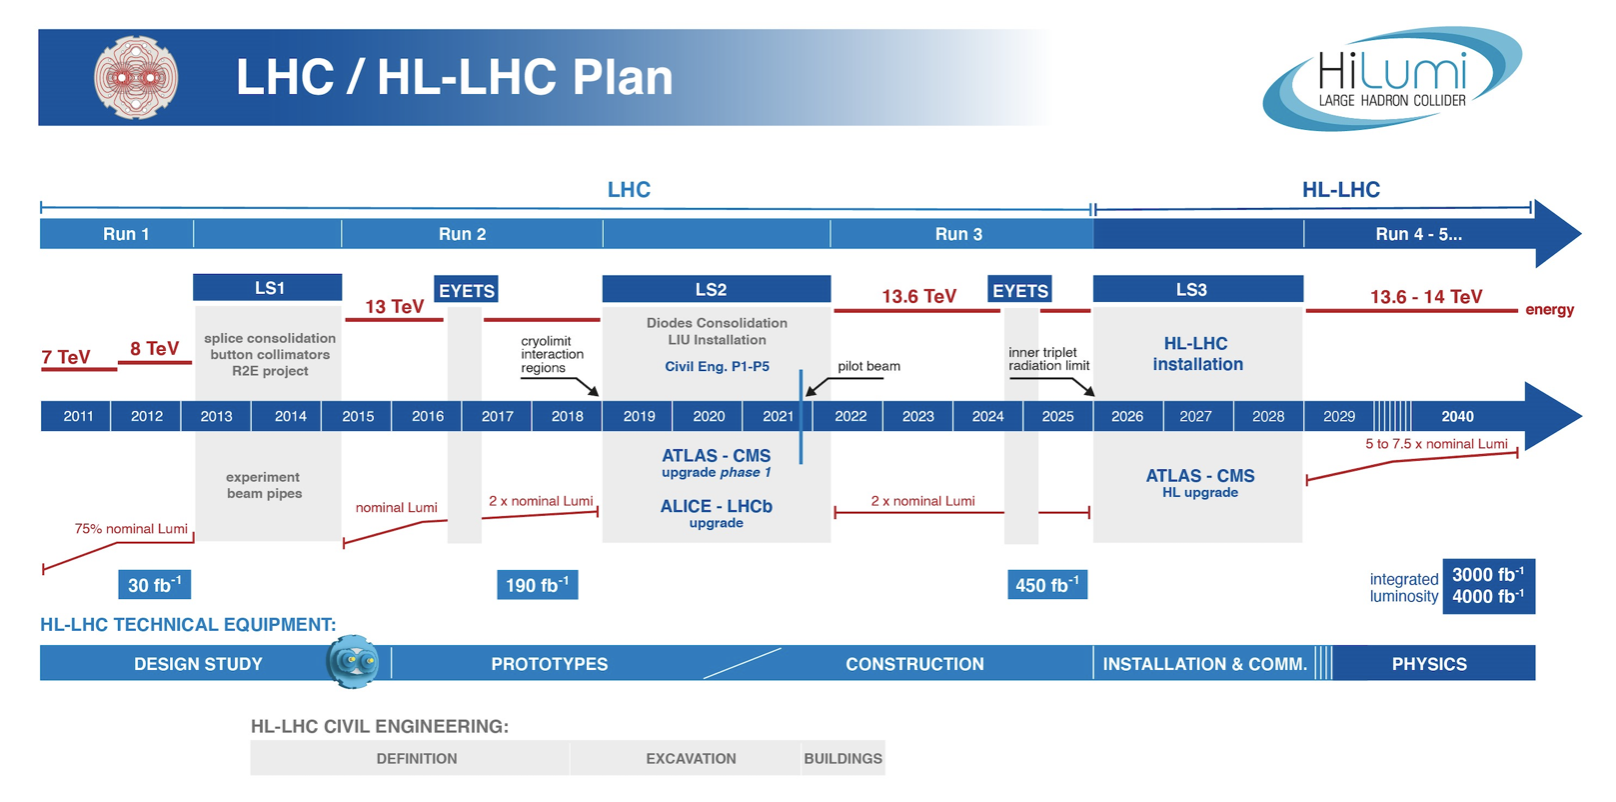
\includegraphics[width=0.9\textwidth]{figures/ch2/hl_lhc_timeline.png}
	\caption{Timeline of LHC activities \cite{lhc_timeline}}
	\label{fig:lhc_timeline}
\end{figure}

 \section{Accelerator Physics}
 \subsection{The Journey of a Proton}
 Protons which feed the LHC start as hydrogen gas. The electrons are removed from the hydrogen atoms through the use of strong electric fields. The linear accelerator (LINAC) then accelerates the $H^-$ ions to an energy of 50 MeV. From here the $H^-$ ions enter the Proton Synchrotron booster, where they are accelerated up to 1.4 GeV of energy. Subsequently they are sorted into bunches separated in time by 25 ns,  where each bunch contains approximately $10^{11}$ protons. Next the bunches pass through the Proton Synchrotron (PS) and the Super Proton Synchrotron (SPS), where they reach energies of 25 GeV and 450 GeV respectively. Finally they are injected into the LHC as two beams traveling in opposite direction. The original design allowed each beam to be accelerated up to 7 TeV of energy. Due to limitations with the magnet training, the highest energy actually achieved by the LHC beams during Run 2 was 6.5 TeV, giving a collision center-of-mass energy of $\sqrt{s}$ = 13 TeV \cite{lhc_faq}. Figure \ref{fig:accelerator_complex} shows the full LHC accelerator complex.\\

\begin{figure}
	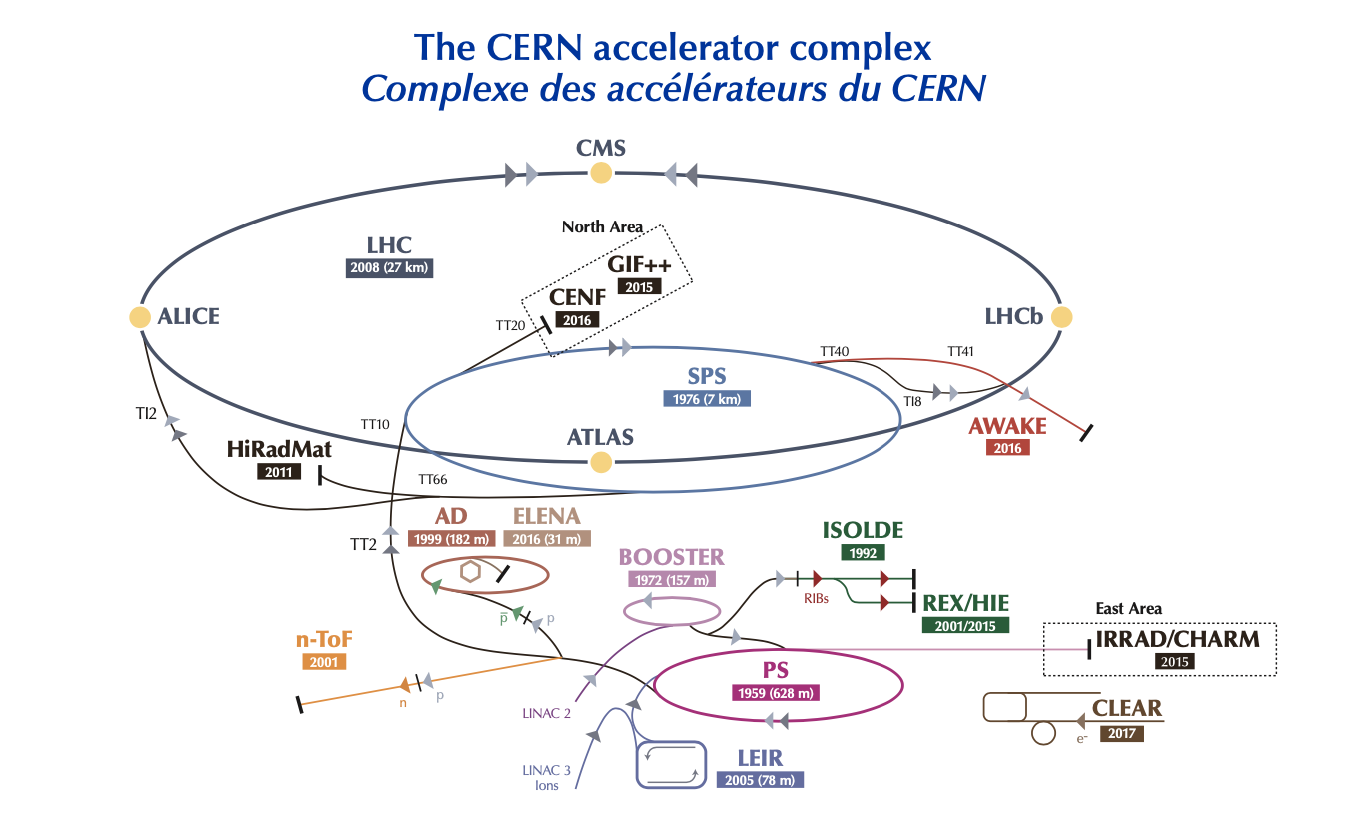
\includegraphics[width=\textwidth]{figures/ch2/accelerator_complex.png}
	\caption{The LHC accelerator complex at CERN \cite{cern_accelerator_complex}}
	\label{fig:accelerator_complex}
\end{figure}

 Acceleration in the LHC is performed by eight radio frequency (RF) cavities located around the ring. Each RF cavity produces a 2MV electric field oscillating at 40 MHz. The 40MHz oscillation produces a point of stable equilibrium every 2.5ns. These points of equilibrium are synchronized with the occurrence of the proton bunches produced in the PS -- a proton bunch occupies one out of every ten points of stable equilibrium, such that the bunches maintain a 25ns spacing \cite{lhc_faq}. \\

\subsection{Magnets}
In addition to the acceleration cavities, the LHC houses 9593 superconducting magnets which direct and focus the proton beam on its 27 kilometer journey. The magnets are comprised of superconducting Niobium-Titanium coils cooled to 1.9K by superfluid helium. As the beams approach one of the four collision points around the ring, multipole magnets focus and squeeze the beam for optimal collisions \cite{lhc_faq}.

The LHC is divided into sections, where each section contains an a smoothly curving \textit{arc} and a straight \textit{insertion}. The arcs are composed of 1232 large dipole magnets which bend the beam to follow the roughly circular 27 km path. The main dipoles generate powerful 8.3 tesla magnetic fields to achieve this bend. Each dipole magnet is 15 meters long and weighs 35 tonnes. The dipoles work in conjunction with quadrupole magnets, which keep the particles in a focused beam, and smaller sextupole, octupole and decapole magnets which tune the magnetic field at the ends of the dipole magnets \cite{lhc_magnets}.

The straight insertion sections have different purposes depending on their location around the ring: beam collisions, beam injection, beam dumping, or beam cleaning. At the four collision points, insertion magnets squeeze the beam to ensure a highly focused collision. This is accomplished with a triplet of quadrupole magnets, which tighten the beam from 0.2 millimeters to just 16 micrometers in diameter. Insertion magnets also clean the beam, which prevents stray particles from hitting sensitive components throughout the LHC. When the LHC is ready to dispose of a beam of particles, beam dump magnets deflect the path of the beam into a straight line towards a block of concrete and graphite that stops the beam. A dilution magnet then reduces the beam intensity by a factor of 100,000 before the final stop \cite{lhc_magnets}. Figure \ref{fig:lhc_octants} shows the locations various beam activities.

\begin{figure}
        \centering
	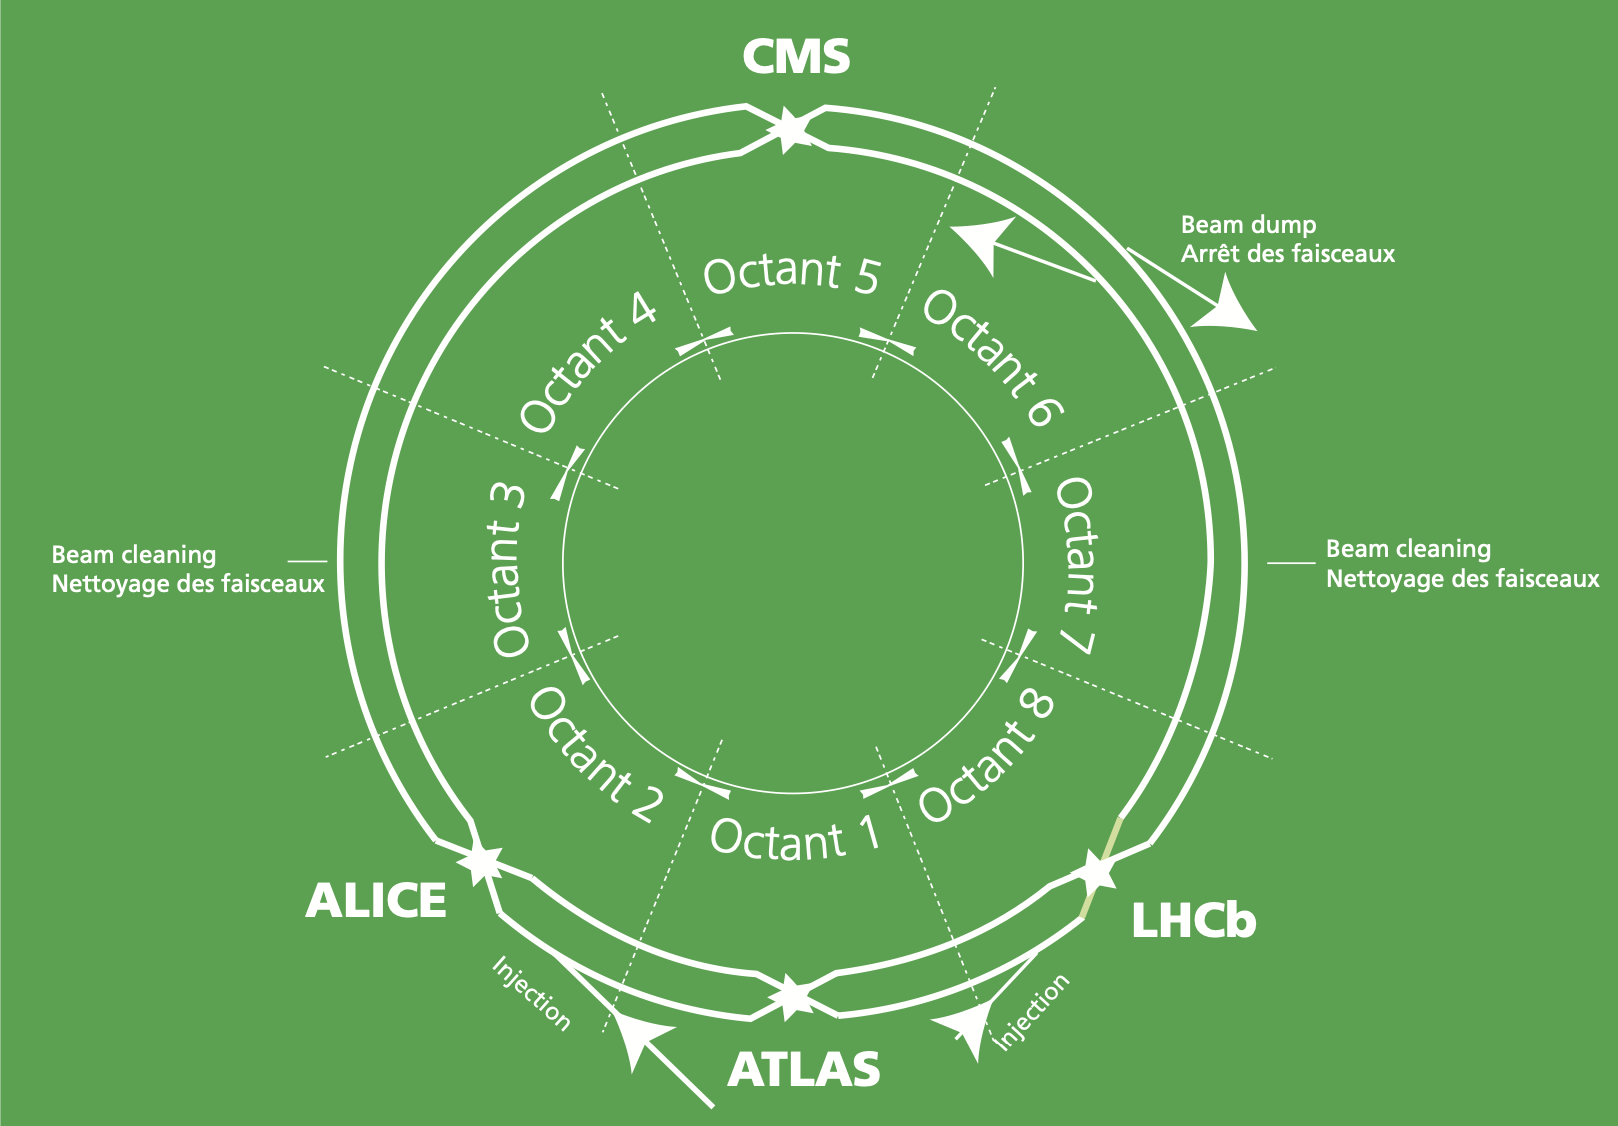
\includegraphics[width=.7\textwidth]{figures/ch2/lhc_octants.png}
	\caption{The octants of the LHC and location of various beam activities \cite{lhc_faq}}
	\label{fig:lhc_octants}
\end{figure} 
 
 \section{Luminosity}
 
Collisions at the LHC occur when the two beams of proton bunches cross at one of the four interaction points. The intensity of collisions is described by the instantaneous luminosity, the formula for which is given in equation \ref{eq:lumi}.  
 \begin{equation}
	L = \frac{f N_1 N_2}{4 \pi \sigma_x \sigma_y}
	\label{eq:lumi}
\end{equation}

Here $f$ is the revolution frequency, $N_1$ and $N_2$ are the number of particle per bunch for each beam, and $\sigma_x$, $\sigma_y$ are the horizontal and vertical beam widths. \\

The instantaneous luminosity gives the number of the collisions that could be produced at the interaction point per cm\textsuperscript{2} of cross-sectional area per second. The integrated luminosity is obtained by integrating the instantaneous luminosity over a given block of time, and measures the total number of collisions which has occurred during that operation period. This is directly correlated with the size of the datasets collected by the LHC experiments.\\
 
 The design peak luminosity of the LHC is $1.0 \times 10^{34}$ cm\textsuperscript{-2}s\textsuperscript{-1}. During Run 1 of the LHC the peak instantaneous luminosity was $0.8 \times 10^{34}$ cm\textsuperscript{-2}s\textsuperscript{-1}. Over the course of Run 1 the LHC collected a total integrated luminosity of 5.46 \invfb at $\sqrt{s} = 7$ TeV, and 22.8 \invfb at $\sqrt{s} = 8$ TeV. Following the first long shutdown and upgrade phase of operations, the LHC achieved a center of mass energy $\sqrt{s} = 13$ TeV at the beginning of Run 2 in 2015. The LHC was also able to deliver $2.0 \times 10^{34}$ cm\textsuperscript{-2}s\textsuperscript{-1} peak instantaneous luminosity, double the design value. During LHC Run 2, from 2015-2018, the LHC delivered 156 \invfb of integrated luminosity for proton-proton collisions. Run 3 of the LHC began in 2022, and is expected to deliver $250$ \invfb of integrated luminosity to the ATLAS and CMS experiments by 2026 \cite{lhc_timeline}.\\
 
The goal of LHC physic analyses is to find and study rare events produced by interesting physics processes. The cross section $\sigma$ of a given process indicates the probability of that process occurring given the beam conditions of the LHC. Multiplying the cross section by the integrated luminosity of a dataset gives the expected number of events for that process within the dataset.

 \begin{equation}
	N\textsubscript{events} = \int \sigma L(t) dt = \mathcal{L} \times \sigma
	\label{eq:xs}
\end{equation}

The cross section for most processes of interest, especially BSM processes, is several orders of magnitude below the total cross section for the LHC. Therefore maximizing the number of events produced in collisions is crucial to increase the likelihood of producing events from processes of interest. For this reason, maximizing instantaneous luminosity is a key factor in accelerator design and operation.
